\chapter{Metodologia}
\label{cap:metodologia}

A arquitetura proposta na Figura \ref{fig:estrutura} fundamenta-se na integração de quatro componentes principais organizados de forma modular para proporcionar uma solução completa para controle de nível industrial distribuída.

\begin{figure}[H]
    \centering
    \caption[Arquitetura do sistema de controle de nível com lógica Fuzzy integrado via OPC UA.]{Arquitetura do sistema de controle de nível com lógica Fuzzy integrado via OPC UA.}
    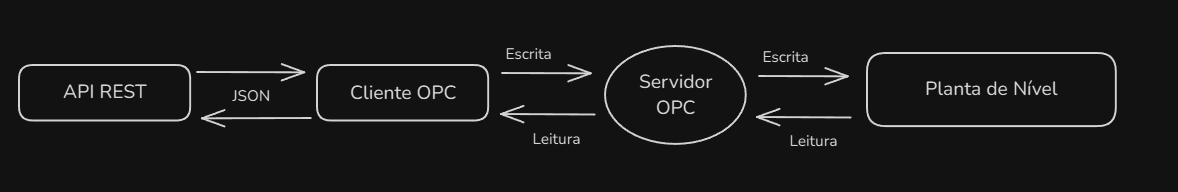
\includegraphics[width=1\textwidth]{figuras/imagens/estrutura.png}
    \label{fig:estrutura}
    \footnotesize Fonte: Dias, 2025. % Ajuste para a fonte
\end{figure}

\begin{itemize}
\item Planta de nível simulada (Matlab/Simulink): Elemento central do sistema representando o processo industrial a ser controlado. Desenvolvida no ambiente Matlab/Simulink.
\item API REST de controle Fuzzy: Núcleo inteligente responsável pela implementação dos algoritmos de controle baseados em lógica Fuzzy.
\item Cliente OPC UA integrado com IHM: Componente intermediário que estabelece comunicação segura via protocolo OPC UA. Responsável pela leitura periódica das variáveis de processo, consumo da API de controle Fuzzy através de requisições HTTP e escrita dos sinais de controle. Integra uma IHM intuitiva para visualização em tempo real, monitoramento, configuração e intervenção manual.
\item Desenvolvimento da interface humano-máquina: Criar uma IHM (Interface Humano-Máquina) intuitiva e funcional que permita a configuração dinâmica da API e do cliente OPC, bem como a visualização em tempo real do controle de nível, proporcionando monitoramento eficiente e facilidade de operação do sistema integrado.
\item Servidor OPC: Ponte de comunicação que expõe as variáveis da planta simulada no espaço de endereçamento OPC. Disponibiliza variáveis garantindo interoperabilidade, segurança e escalabilidade.
\end{itemize}

\section{Escolha da planta de nível}
\label{sec:escolhaplanta}

Para o presente trabalho foi selecionada a planta de nível de água em tanque disponível como exemplo no conjunto de bibliotecas do Matlab, especificamente o modelo `sltank`. Esta escolha justifica-se pelo fato de que a proposta do trabalho é o desenvolvimento da integração entre sistemas e não a parametrização de uma nova planta de nível, além de permitir validação com uma referência estabelecida na literatura técnica.

O sistema de controle de nível de água em tanque apresenta características não lineares típicas de processos industriais reais. O controle é realizado através de uma válvula que regula o fluxo de entrada de água no tanque, enquanto a vazão de saída depende do diâmetro do tubo de saída (constante) e da pressão no tanque, que varia proporcionalmente ao nível de água. Esta característica confere ao sistema comportamento dinâmico não linear, tornando-o adequado para demonstrar as vantagens da aplicação de técnicas de controle inteligente.

O sistema de controle de nível apresenta as seguintes variáveis principais:

Variáveis de entrada do controlador Fuzzy:

\begin{itemize}
\item level (erro de nível): Diferença entre o nível desejado (setpoint) e o nível atual de água no tanque, medida em unidades de altura. Esta variável representa o desvio que o sistema deve corrigir para manter o nível na referência estabelecida.
\item rate (taxa de variação do nível): Derivada temporal do nível de água, indicando a velocidade de variação do nível no tanque. Esta variável fornece informação sobre a tendência de comportamento do sistema, permitindo ações antecipativas do controlador.
\end{itemize}

Variável de saída do controlador Fuzzy:

\begin{itemize}
\item valve (sinal de controle da válvula): Taxa de abertura ou fechamento da válvula de controle de entrada, expressa em percentual ou unidades normalizadas. Este sinal determina a vazão de entrada de água no tanque, constituindo a ação de controle aplicada ao processo.
\end{itemize}

A representação da planta está definida conforme a Figura \ref{fig:planta}.

\begin{figure}[H]
    \centering
    \caption[Planta de nível de água em tanque do Matlab/Simulink (modelo sltank).]{Planta de nível de água em tanque do Matlab/Simulink (modelo sltank).}
    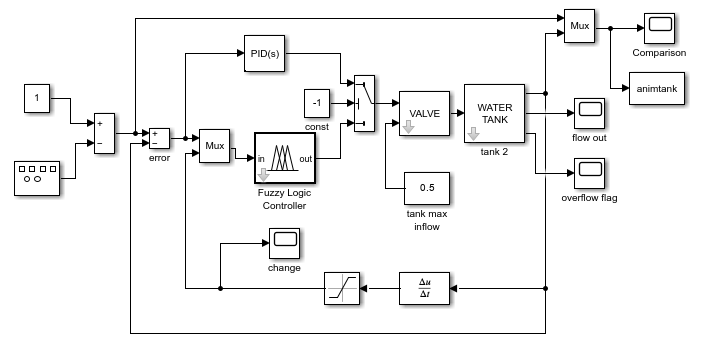
\includegraphics[width=1\textwidth]{figuras/imagens/plantamatlab.png}    
    {Fonte: Dias, 2025.}
    \label{fig:planta}
\end{figure}

\section{API de controle Fuzzy}
\label{sec:apifuzzy}

A implementação da API de controle Fuzzy constitui o núcleo inteligente do sistema proposto, responsável pela execução dos algoritmos de lógica Fuzzy que determinam as ações de controle aplicadas à planta de nível. A escolha da linguagem Python para o desenvolvimento desta API justifica-se por sua ampla disponibilidade de bibliotecas especializadas em sistemas Fuzzy, facilidade de desenvolvimento de APIs REST e capacidade de integração com diferentes tecnologias.

A API segue o padrão arquitetural REST (Representational State Transfer), proporcionando interface padronizada para integração com a IHM. Esta abordagem garante flexibilidade na comunicação, permitindo que diferentes clientes possam consumir os serviços de controle independentemente da plataforma ou tecnologia utilizada. A estrutura modular permite separação clara entre a lógica de controle Fuzzy e a interface de comunicação, facilitando manutenção e futuras expansões do sistema.

O controlador Fuzzy utiliza a parametrização extraída da planta de nível do Matlab (modelo `sltank`), adaptada para implementação em Python. Esta escolha metodológica assegura compatibilidade com a literatura técnica existente e permite validação dos resultados através de comparação com implementações de referência. A API implementa duas variáveis de entrada (erro de nível e taxa de variação) e uma variável de saída (sinal de controle da válvula), utilizando funções de pertinência triangulares e trapezoidais com universos de discurso normalizados.

A base de regras implementada contempla 49 regras de inferência (matriz 7x7), desenvolvidas com base no conhecimento heurístico sobre comportamento de sistemas de controle de nível. A estratégia de controle privilegia ação corretiva proporcional ao erro, comportamento antecipativo baseado na taxa de variação e estabilização para pequenos desvios.

\section{Desenvolvimento da IHM}
\label{sec:devihm}

O desenvolvimento da Interface Humano-Máquina (Figura 3) constitui o componente de interação e supervisão do sistema integrado, proporcionando visualização em tempo real, monitoramento das variáveis de processo e capacidade de intervenção manual no sistema de controle. A escolha da linguagem C-Sharp para o desenvolvimento da IHM justifica-se por sua robustez na criação de aplicações desktop, ampla disponibilidade de bibliotecas para comunicação OPC UA e facilidade de integração com APIs REST.

A representação da IHM está definida conforme a Figura \ref{fig:ihm}.

\begin{figure}[H]
    \centering
    \caption[Interface Humano-Máquina desenvolvida em C\# para supervisão e controle.]{Interface Humano-Máquina desenvolvida em C\# para supervisão e controle.}
    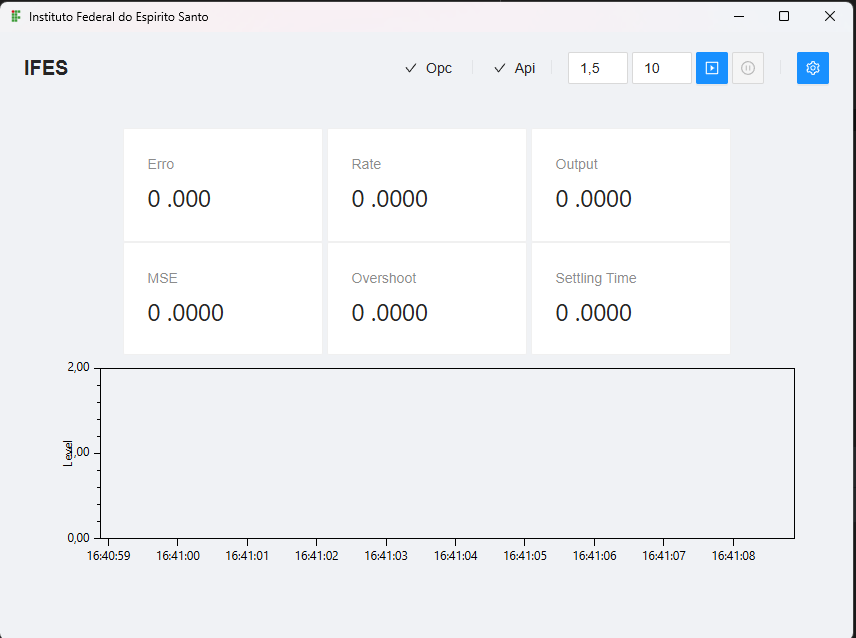
\includegraphics[width=1\textwidth]{figuras/imagens/ihm.png}    
    {Fonte: Dias, 2025.}
    \label{fig:ihm}
\end{figure}

A IHM segue uma arquitetura cliente-servidor, atuando simultaneamente como cliente OPC UA para comunicação com a planta simulada e cliente HTTP para consumo da API de controle Fuzzy. Esta abordagem dual permite que a aplicação funcione como elemento centralizador da arquitetura, coordenando o fluxo de dados entre todos os componentes do sistema. A estrutura modular facilita a manutenção e permite expansões futuras sem comprometer a funcionalidade existente.

A aplicação implementa comunicação bidirecional com o servidor OPC UA, realizando leitura periódica das variáveis de processo (nível atual, setpoint e sinais de controle) e escrita dos comandos de controle calculados pela API Fuzzy. Esta integração utiliza bibliotecas especializadas em OPC UA para C-Sharp, garantindo conformidade com os padrões industriais e compatibilidade com diferentes servidores OPC. A configuração das tags OPC é realizada de forma dinâmica, permitindo adaptação a diferentes configurações de planta sem necessidade de recompilação.

A interface gráfica proporciona visualização intuitiva das variáveis de processo através de gráficos em tempo real, indicadores visuais de status e controles para configuração de parâmetros operacionais. A aplicação implementa funcionalidades de monitoramento contínuo, registro de dados históricos e alarmes para condições de operação anômalas. A integração com a API de controle Fuzzy é realizada através de requisições HTTP periódicas, enviando as variáveis de processo e recebendo os sinais de controle calculados, garantindo operação em tempo real adequada para aplicações de controle industrial.

\section{Integração e Testes}
\label{sec:intetestes}

A metodologia de integração e testes constitui a fase de validação do sistema integrado, responsável por verificar a eficácia da arquitetura proposta através da avaliação do desempenho do controle Fuzzy distribuído via protocolo OPC UA. Esta etapa metodológica visa demonstrar a viabilidade da integração entre sistemas heterogêneos mantendo ou superando o desempenho de controle obtido com implementações convencionais.

A estratégia de integração segue uma abordagem incremental, iniciando com testes unitários de cada componente individual, progredindo para testes de integração entre pares de componentes e culminando com a validação do sistema completo. Esta metodologia garante identificação precoce de problemas de compatibilidade e permite refinamento progressivo da arquitetura antes dos testes finais de desempenho.

\begin{itemize}
\item Testes de componentes individuais: Validação isolada da API de controle Fuzzy, verificação da funcionalidade da IHM, teste de comunicação OPC UA entre servidor e cliente, e confirmação da estabilidade da planta simulada. Esta fase assegura que cada elemento funcione corretamente antes da integração.
\item Testes de integração por pares: Verificação da comunicação entre IHM e API Fuzzy via HTTP, validação da troca de dados entre IHM e servidor OPC UA, e teste da sincronização temporal entre os componentes. Esta etapa identifica problemas de interface e protocolo de comunicação.
\item Testes de sistema completo: Avaliação do desempenho de controle com todos os componentes integrados, medição de latências de comunicação, verificação da robustez do sistema a falhas temporárias de comunicação, e análise da estabilidade em operação contínua prolongada.
\end{itemize}

A metodologia de avaliação de desempenho baseia-se na comparação entre duas configurações de controle: o sistema integrado proposto (API Fuzzy distribuída via OPC UA) e o sistema de referência (controlador Fuzzy nativo do Matlab aplicado diretamente à planta). Esta abordagem comparativa permite quantificar o impacto da arquitetura distribuída no desempenho de controle.

Critérios de avaliação estabelecidos:

\begin{itemize}
\item Estabilidade: Capacidade do sistema de manter controle estável sem oscilações persistentes.
\item Tempo de acomodação: intervalo necessário para que a resposta do sistema atinja e permaneça dentro de 2\% do valor final.
\item Precisão em regime permanente: Desvio percentual entre o valor desejado e o valor alcançado em estado estacionário.
\item Latência de comunicação: Tempo de resposta da arquitetura distribuída comparado ao sistema centralizado.
\end{itemize}
